\subsection{BMP085 Trykføler}

I forbindelse med læsning af sensordata fra den barometriske trykmåler BMP085, bruges I2C interfacet. Atmega32 understøtter I2C komunikatiuon og på figur~\ref{fig:voltagedivider} ses den hardwaremæssige opsætning. Atmega 32’s input spænding er 5V bruges en simpel spændingsdeler, så BMP085 ikke overbelastes.


\begin{figure}[h]
	\centering
	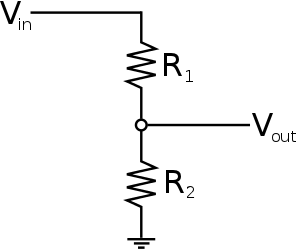
\includegraphics[width=0.4\linewidth]{figs/voltage_divider}
	\caption{Spændingsdeler.}
	\label{fig:voltagedivider}
\end{figure}

På figur~\ref{fig:voltagediv} vise modstandsberegningerne til spændingsdeleren.



\begin{figure}[h]
	\centering
	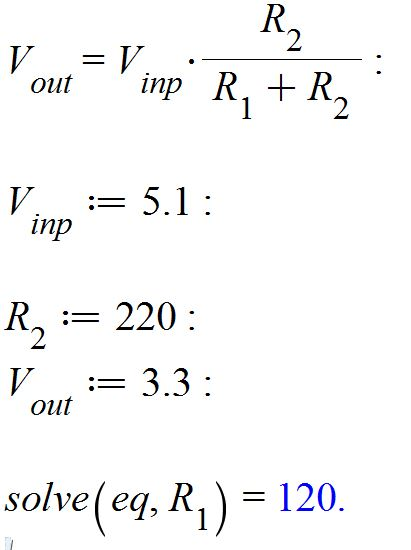
\includegraphics[width=0.3\linewidth]{figs/voltage_div}
	\caption{Spændingsdeler.}
	\label{fig:voltagediv}
\end{figure}

\subsection{Brug af I2C bussen med BMP085}

I2C protokollen implementerer master/slave teknikken, og er et TWI (two wire interface). 
Atmega32 agerer I2C master som sætter clock hastigheden ved at skrive til PIN (SCK). I2C masteren sender data bytes til I2C slaven på addressen 0x77.
Ifølge BMP085’s datablad er følgene kommandoer mulige:

\begin{figure}[h]
	\centering
	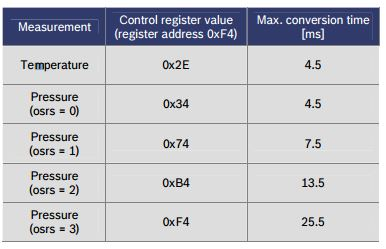
\includegraphics[width=0.6\linewidth]{figs/bmp085_commands}
	\caption{BMP085 kommandoer.}
	\label{fig:bmp085commands}
\end{figure}

Kommandoerne er definerede BMP085 driverens h-fil. Oversampling modes er defineret separat.

\begin{figure}[h]
	\centering
	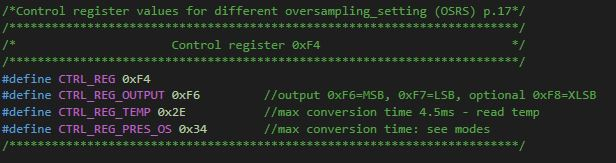
\includegraphics[width=0.7\linewidth]{figs/bmp085_command_defines}
	\caption{BMP kommandodefinitioer.}
	\label{fig:bmp085commanddefines}
\end{figure}

\begin{figure}[h]
	\centering
	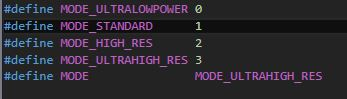
\includegraphics[width=0.7\linewidth]{figs/bmp085_command_modes}
	\caption{BMP085 kommendo tilstande.}
	\label{fig:bmp085commandmodes}
\end{figure}

Timing diagrammet for start af temperatur/tyk måling fremgår a BM085’s datablad, og kan ses på figur~\ref{fig:bmpi2ctiming}.

\begin{figure}[h]
	\centering
	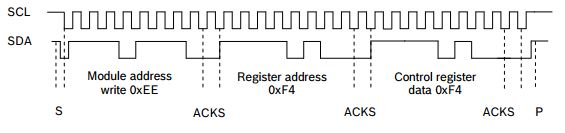
\includegraphics[width=0.9\linewidth]{figs/bmp_i2c_timing}
	\caption{BMM/I2C timingdiagram}
	\label{fig:bmpi2ctiming}
\end{figure}

Som det kan ses på figur~\ref{fig:bmpi2ctiming}, sender BMP085 en ACK for hver 8 bit der modtages. Atmega32 masteren sender en stop condition efter sidste ACK. S indikerer start conditionen.
Som angivet på figur~\ref{fig:bmp085commands} er der konverterings tider forbundet med målingerne. BMP085 giver muliged for at signalere et fuldendt måling ved at sætte BMP085’s EOC pin høj når en kovertering er slut. Dette bruges dog ikke i dette projekt da der ikke har været tid til at udvikle kredsløbet der hiver 3.3v logik op til 5v.


% The technical considerations and choices made during the project work.

% Advantages and disadvantages for the possible alternative solutions.

% How the group has acquired the knowledge necessary to do the project work.
